\documentclass{article}

\usepackage{fancyhdr}
\usepackage{extramarks}
\usepackage{amsmath}
\usepackage{amsthm}
\usepackage{amsfonts}
\usepackage{amssymb}
\usepackage{xparse}
\usepackage{tikz}
\usepackage{graphicx}
\usepackage[plain]{algorithm}
\usepackage{algpseudocode}
\usepackage{listings}
\usepackage{hyperref}
\usepackage[per-mode = fraction]{siunitx}
\usepackage{calc}

\usetikzlibrary{automata,positioning}

\hypersetup{
    colorlinks=true,
    linkcolor=blue,
    filecolor=magenta,
    urlcolor=blue,
    }

\urlstyle{same}

%
% Basic Document Settings
%

\topmargin=-0.45in
\evensidemargin=0in
\oddsidemargin=0in
\textwidth=6.5in
\textheight=9.0in
\headsep=0.25in

\linespread{1.1}

\pagestyle{fancy}
\lhead{\hmwkAuthorName}
\chead{\hmwkClass\ (\hmwkClassInstructor,\ \hmwkClassTime): \hmwkTitle}
\rhead{\firstxmark}
\lfoot{\lastxmark}
\cfoot{\thepage}

\renewcommand\headrulewidth{0.4pt}
\renewcommand\footrulewidth{0.4pt}

\setlength\parindent{0pt}
\allowdisplaybreaks
%
% Title Page
%

\title{
	\vspace{2in}
	\textmd{\textbf{\hmwkClass:\ \hmwkTitle}}\\
	\normalsize\vspace{0.1in}\small{Due\ on\ \hmwkDueDate\ at \hmwkDueTime}\\
	\vspace{0.1in}\large{\textit{\hmwkClassInstructor,\ \hmwkClassTime}}
	\vspace{3in}
}
\author{\textbf{\hmwkAuthorName}}
\date{\hmwkCompletionDate}

%
% Create Problem Sections
%

\newcommand{\enterProblemHeader}[1]{
	\nobreak\extramarks{}{Problem #1 continued on next page\ldots}\nobreak{}
	\nobreak\extramarks{Problem #1 (continued)}{Problem #1 continued on next page\ldots}\nobreak{}
}

\newcommand{\exitProblemHeader}[1]{
	\nobreak\extramarks{Problem #1 (continued)}{Problem #1 continued on next page\ldots}\nobreak{}
	\nobreak\extramarks{Problem #1}{}\nobreak{}
}

%
% Homework Problem Environment
%
\NewDocumentEnvironment{hwkProblem}{m m s}{
	\section*{Problem #1: #2}
	\enterProblemHeader{#1}
	\setcounter{partCounter}{1}
}{
	\exitProblemHeader{#1}
	\IfBooleanF{#3} % if star, no new page
		{\newpage}
}

% Alias for the Solution section header
\newcommand{\hwkSol}{\vspace{\baselineskip / 2}\textbf{\Large Solution}\vspace{\baselineskip / 2}}

% Alias for the Solution Part subsection header
\newcounter{partCounter}
\newcommand{\hwkPart}{
	\vspace{\baselineskip / 2}
	\textbf{\large Part \Alph{partCounter}}
	\vspace{\baselineskip / 2}
	\stepcounter{partCounter}
}

%
% Various Helper Commands
%

% Such That
\newcommand{\st}{\text{s.t.}}

% Useful for algorithms
\newcommand{\alg}[1]{\textsc{\bfseries \footnotesize #1}}

% For derivatives
\newcommand{\deriv}[1]{\frac{\mathrm{d}}{\mathrm{d}x} (#1)}

% For partial derivatives
\newcommand{\pderiv}[2]{\frac{\partial}{\partial #1} (#2)}

% Integral dx
\newcommand{\dx}{\mathrm{d}x}
\newcommand{\dy}{\mathrm{d}y}

% Probability commands: Expectation, Variance, Covariance, Bias
\newcommand{\e}[1]{\mathrm{e}#1}
\newcommand{\E}{\mathrm{E}}
\newcommand{\Var}{\mathrm{Var}}
\newcommand{\Cov}{\mathrm{Cov}}
\newcommand{\Bias}{\mathrm{Bias}}

% Defining Units that are not in the SI base
\DeclareSIUnit\bar{bar}
\DeclareSIUnit\ft{ft}
\DeclareSIUnit\dollar{\$}
\DeclareSIUnit\cent{\text{\textcent}}
\DeclareSIUnit\c{\degreeCelsius}

% Code Listing config
\usepackage{xcolor}
\definecolor{codegreen}{rgb}{0,0.6,0}
\definecolor{codegray}{rgb}{0.5,0.5,0.5}
\definecolor{codepurple}{rgb}{0.58,0,0.82}
\definecolor{backcolour}{rgb}{0.95,0.95,0.92}
\lstdefinestyle{overleaf}{
	% backgroundcolor=\color{backcolour},
	commentstyle=\color{codegreen},
	keywordstyle=\color{magenta},
	numberstyle=\tiny\color{codegray},
	stringstyle=\color{codepurple},
	basicstyle=\ttfamily\footnotesize,
	breakatwhitespace=false,
	breaklines=true,
	captionpos=b,
	keepspaces=true,
	numbers=left,
	numbersep=5pt,
	showspaces=false,
	showstringspaces=false,
	showtabs=false,
	tabsize=4
}

\usepackage[latte]{catppuccinpalette}
\lstdefinestyle{catppuccin}{
	breaklines=true,
	keepspaces=true,
	numbers=left,
	numbersep=5pt,
	showspaces=false,
	showstringspaces=false,
	breakatwhitespace=true,
	tabsize=4,
	stringstyle = {\color{CtpGreen}},
	commentstyle={\color{CtpOverlay1}},
	basicstyle = {\small\color{CtpText}\ttfamily},
	keywordstyle = {\color{CtpMauve}},
	keywordstyle = [2]{\color{CtpBlue}},
	keywordstyle = [3]{\color{CtpYellow}},
	keywordstyle = [4]{\color{CtpLavender}},
	keywordstyle = [5]{\color{CtpPeach}},
	keywordstyle = [6]{\color{CtpTeal}}
}

\lstset{style=catppuccin}


%
% Homework Details
%   - Title
%   - Subtitle
%   - Due date
%   - Due time
%   - Course
%   - Section/Time
%   - Instructor
%   - Author
%

\newcommand{\hmwkTitle}{HW 06}
\newcommand{\hmwkSubTitle}{Assignment 6}
\newcommand{\hmwkDueDate}{March 13th, 2025}
\newcommand{\hmwkDueTime}{11:59 PM}
\newcommand{\hmwkClass}{PHYS 313}
\newcommand{\hmwkClassTime}{0101}
\newcommand{\hmwkClassInstructor}{Dr.\ Ji}
\newcommand{\hmwkAuthorName}{\textbf{Vai Srivastava}}
\newcommand{\hmwkCompletionDate}{\today}

\begin{document}

\maketitle

\pagebreak

\begin{hwkProblem}{3.2}{}

	In one sentence, justify Earnshaw's Theorem.

	\hwkSol{}

\end{hwkProblem}
\begin{hwkProblem}{3.3}{}

	Find the general solution to Laplace's equation in spherical coordinates, for the case where \( V \) depends only on \( r \). Do the same for cylindrical coordinates, assuming \( V \) depends only on \( s \).

	\hwkSol{}

\end{hwkProblem}
\begin{hwkProblem}{3.4}{}

	\begin{enumerate}
		\item Show that the average electric field over a spherical surface, due to charges outside the sphere, is the same as the field at the center.
		\item What is the average due to charges inside the sphere?
	\end{enumerate}

	\hwkSol{}

\end{hwkProblem}
\begin{hwkProblem}{3.7}{}

	Find the force on the charge \( +q \) in the below image, noting that the \( xy \) plane is a grounded conductor.
	\begin{figure}[H]
		\begin{center}
			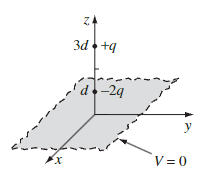
\includegraphics[width=0.35\textwidth]{./images/p3_7.png}
		\end{center}
		\caption{Diagram for Problem 3.7}\label{fig:p3_7}
	\end{figure}

	\hwkSol{}

\end{hwkProblem}
\begin{hwkProblem}{3.8}{}

	\begin{enumerate}
		\item Using the law of consines, show that the following equations are equivalent:
			\begin{align}
				\func{V}[\vecb{r}] &= \frac{1}{4 \pi \epsilon_{0}} \left( \frac{q}{\rcurs} + \frac{q'}{\rcurs '} \right) \\
				\func{V}[r, \theta] &= \frac{1}{4 \pi \epsilon_{0}} \left[ \frac{q}{\sqrt{r^{2}+a^{2}-2ra\cos\left(\theta\right)}} - \frac{q}{\sqrt{R^{2}+{\left(\frac{ra}{R}\right)}^{2}-2ra\cos\left(\theta\right)}} \right]
			\end{align}
			Where \( r \) and \( \theta \) are the usual spherical polar coordinates, with the \( z \) axis along the line through \( q \). In this form, it is obvious that \( V = 0 \) on the sphere \( r = R \).
		\item Find the induced surface charge on the sphere, as a function of \( \theta \). Integrate this to get the total induced charge. (What \textit{should} it be?)
		\item Calculate the energy of this configuration.
	\end{enumerate}

	\hwkSol{}

\end{hwkProblem}
\begin{hwkProblem}{3.13}{}
	
	Find the potential in the infinite slot of Ex3.3 if the boundary at \( x = 0 \) consists of two metal strips: one, from \( y = 0 \) to \( y = \frac{a}{2} \), is held at a constant potential \( V_{0} \), and the other, from \( y = \frac{a}{2} \) to \( y = a \), is at potential \( -V_{0} \).

	\hwkSol{}

	Similar to the answer in Ex3.3, the configuration retains its independence from \( z \). We again have to solve Laplace's equation but subjected to different boundary conditions:
	\[
		\pderivsec{x}{V} + \pderivsec{y}{V} = 0,
		\begin{cases}
			V = 0 & y = 0 \\
			V = 0 & y = a \\
			V = V_{0} & 0 < y < \frac{a}{2}, x = 0 \\
			V = -V_{0} & \frac{a}{2} < y < a, x = 0 \\
			V \to 0 & x \to \infty
		\end{cases}
	.\]
	This can be accomplished using a similar technique as Griffiths, as follows:
	\begin{align*}
		Y \derivsec{x}{X} + X \derivsec{y}{Y} &= 0 \\
		\frac{1}{X} \derivsec{x}{X} + \frac{1}{Y} \derivsec{y}{Y} &= 0 \\
		\derivsec{x}{X} = k^{2}X ,& \quad \derivsec{y}{Y} = -k^{2}Y \\
		\func{X}[x] = Ae^{kx}+Be^{-kx} ,& \quad \func{Y}[y] = C \sin{ky} + D \cos{ky} \\
		\func{V}[x, y] &= \left(Ae^{kx}+Be^{-kx}\right) \left(C \sin{ky} + D \cos{ky}\right) \\
		\text{condition (v)} &\implies A = 0 \\
		\therefore \func{V}[x, y] &= e^{-ky} \left(C \sin{ky} + D \cos{ky}\right) \\
		\text{condition (i)} &\implies D = 0 \\
		\therefore \func{V}[x, y] &= C e^{-ky} \sin{ky} \\
		\text{condition (ii)} &\implies \sin{ka} = 0 \\
		\therefore k &= \frac{n\pi}{a}, \quad n = \left\{1, 2, 3, \dots\right\} \\
		\func{V}[x, y] &= \sum_{n=1}^{\infty}C_{n}e^{-n \pi \frac{x}{a}} \sin{n \pi \frac{y}{a}}
	\end{align*}
	Here is where we diverge from Griffiths' Ex3.3. We want to fulfill our conditions (iii) and (iv) as follows:
	\begin{align*}
		\func{V}[0, 0<y<\frac{a}{2}] &= \sum_{n=1}^{\infty}C_{n}e^{-n \pi \frac{x}{a}} \sin{n \pi \frac{y}{a}} = V_{0}, \\
		\func{V}[0, \frac{a}{2}<y<a] &= \sum_{n=1}^{\infty}C_{n}e^{-n \pi \frac{x}{a}} \sin{n \pi \frac{y}{a}} = -V_{0}.
	\end{align*}

\end{hwkProblem}
\end{document}
